\documentclass[a4paper,12pt]{report}
\usepackage[paper=a4paper]{geometry}
\usepackage{placeins}
\usepackage{graphicx}
\usepackage{amssymb}
\usepackage[justification=centering]{caption}
\usepackage[table,xcdraw]{xcolor}
\graphicspath{{C:\Users\User\Desktop\mipt\phys\lab131}}
\DeclareGraphicsExtensions{.pdf,.png,.jpg}

\usepackage[T2A]{fontenc}
\usepackage[utf8]{inputenc}
\usepackage[english,russian]{babel}
\usepackage{amsmath,amsfonts,amssymb,amsthm,mathtools}
\usepackage{wasysym}
\usepackage{wrapfig}
\author{Выполнил Смирнов Иван и Сапронов Юрий, студент Б02-004}
\title{Отчет по лабораторной работе № 1.3.1 \\[15pt] «Определение модуля Юнга на основе исследования деформаций растяжения и изгиба»}
\date{\today}

\usepackage{ragged2e}
\justifying



\begin{document}

\maketitle

\section*{\Large Аннотация}

Работа заключается в экспериментальном получении значения модуля Юнга. Для этого в первой части эксперимента с помощью прибора Лермантова измеряется зависимость между напряжением и деформацией для одноосного растяжения, а во второй части с помощью перечисленного ниже оборудования измеряется та же зависимость для чистого изгиба.

В работе используются: в первой части - прибор Лермантова, проволока из исследуемого материала, зрительная труба со шкалой, набор грузов, микрометр, рулетка; во второй части - стойка для изгибания балки, индикатор для измерения величины прогиба, набор исследуемых стержней, грузы, линейка, штангенциркуль.

В первой части эксперимента производится растяжение 
, что соответствует одноосному наппряженному состоянию, которое описывается формулой, основанной на эмпирических данных:

\begin{equation}
	\sigma = E \epsilon ,
\end{equation}

где $\sigma$ - напряжение, $E$ - модуль упругости, он же модуль Юнга, $\epsilon$ - деформация, она же в данном случае относительное удлинение.

Во второй части же измерения производят при изгибе балки. Связь между ее прогибом и величиной силы, приложенной посредине между точками опор балки, может быть выражена через модуль Юнга. 



\section*{\Large Одноосное напряжение}



\subsection*{Теоретическая справка}

\begin{figure}[h!]
\begin{minipage}[h!]{0.49\linewidth}
	\center{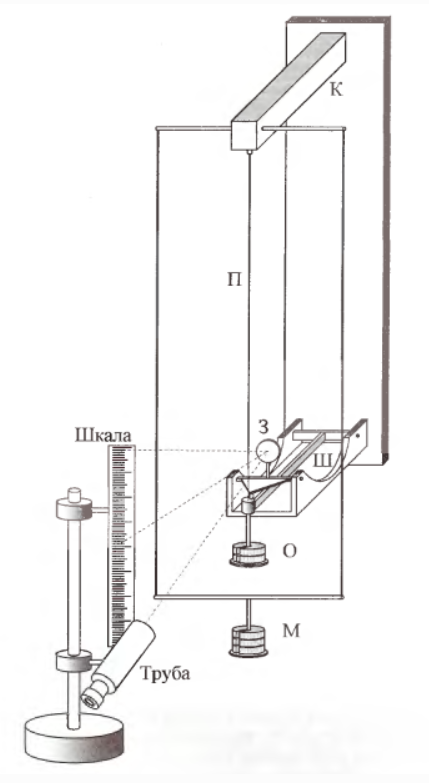
\includegraphics[width=0.5\linewidth]{lab131ris1.png}}
\end{minipage}
\hfill
\begin{minipage}[h!]{0.49\linewidth}
	\center{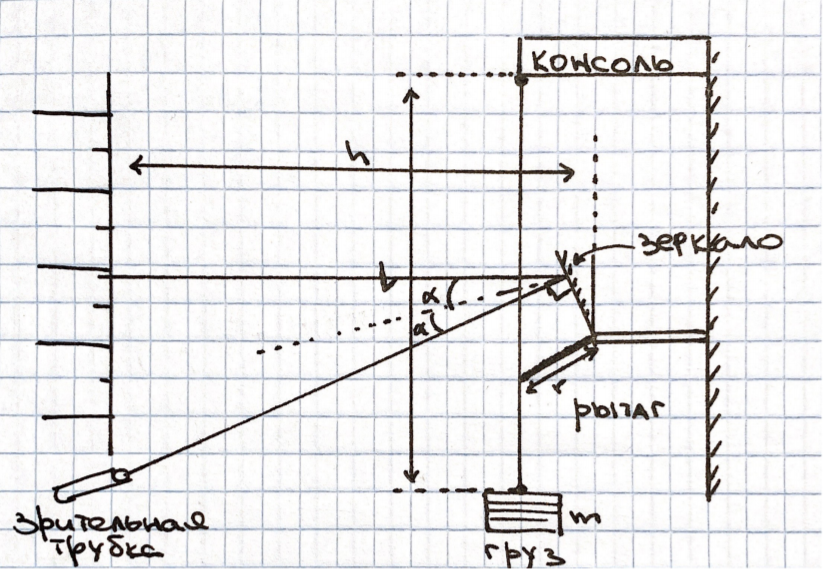
\includegraphics[width=1\linewidth]{lab131ris2.png}}
\end{minipage}
\caption{\textit{$L$ - длина проволоки, $r$ - длина рычага, $\Delta L$ - удлинение проволоки, $\alpha$ - угол отклонения зеркала, $h$ - расстояние от шкалы до зеркала, $\Delta S$ - изменение по шкале.}}
\end{figure}

Запишем закон Гука:

\begin{equation}
	\frac{P}{S}=E\frac{\Delta L}{L},
	\label{form2}
\end{equation}

где $S$ - площадь поперечного сечения проволоки, $P$ - вес нагрузки.

При малых $\Delta L$ угол $\alpha$ также можно считать малым, тогда, пользуясь геометрией установки, распишем тангенс угла между рычагом и горизонталью, который, как может быть видно, также равен углу между лучами из трубки:

\begin{equation}
	2 \alpha = \frac{\Delta L}{r} , \Delta S \approx 2 \alpha h \Rightarrow \Delta L \approx \frac{\Delta S r}{2 h}.
	\label{form3}
\end{equation}

Рассчитаем величину предельной нагрузки, действие которой приводит к необратимой деформации. Она составляет не более $30\%$ от разрушающей равной $900 H/$мм$^2$. То есть, говоря о массе грузов, мы можем навесить не больше $10$ килограмм. Выходит так, что лабораторная установка не позволяет использовать и половины такой нагрузки, поэтому необратимой деформацией мы пренебрегаем.
 


\subsection*{Измерения, погрешности и конечный результат}



Снимем зависимость удлинения проволоки, то есть числа делений n по шкале, от массы грузов $m$ при увеличении и уменьшении нагрузки. Результаты приведем в таблице 2. Усредним измерения для каждой нагрузки и учтем погрешности - таблица 2. Подставим измерения по шкале в формулу $(4)$, рассчитаем погрешности, результаты вынесем в таблицу 3 и на основании них построим график зависимости удлинения проволоки от нагрузки - рисунок 2. На рисунке 2 видим аппроксимирующую прямую, которая была построена по МНК. Коэффициент наклона известен и погрешность рассчитана, вычисления приведены не будут. 

Модуль Юнга будем рассчитывать по следующей формуле:

\begin{equation}
	E = \frac{4kl}{\pi d^2},
	\label{Eodnoos}
\end{equation}

Где $d = 0,73\times 10^{-4}$ м, $l = (17747\pm7)\times 10^{-4}$ м. В результате имеем таблицу 4 с конечными результатами измерения.


\begin{table}[h]
\begin{center}
\begin{tabular}{|c|c|c|}
\hline
Вес   нагрузки, Н & Измерение 1, мм & Измерение 2, мм \\ \hline
4.6               & 16.7            & 16.8            \\ \hline
9.6               & 19.5            & 19.5            \\ \hline
14.6              & 21.3            & 21.6            \\ \hline
19.5              & 23.2            & 23.5            \\ \hline
24.4              & 26.5            & 26.5            \\ \hline
29.3              & 28.9            & 29.1            \\ \hline
24.4              & 26.5            & 26.6            \\ \hline
19.5              & 23.5            & 23.7            \\ \hline
14.6              & 21.5            & 21.6            \\ \hline
9.6               & 19.9            & 20.1            \\ \hline
4.6               & 16.8            & 16.5            \\ \hline
\end{tabular}
\end{center}
\caption{\textit{Измерение изменения на шкале в зависимости от нагрузки.}}
\end{table}

\begin{table}[h!]
\begin{center}
\begin{tabular}{|c|c|c|c|}
\hline
Измерение по шкале, мм & Случайная, мм & Статистическая,мм & Полная, мм \\ \hline
16.7                   & 1.62          & 0.05              & 1.62       \\ \hline
19.8                   & 0.30          & 0.05              & 0.30       \\ \hline
21.5                   & 0.14          & 0.05              & 0.15       \\ \hline
23.5                   & 0.21          & 0.05              & 0.21       \\ \hline
26.5                   & 0.06          & 0.05              & 0.08       \\ \hline
29.0                   & 0.14          & 0.05              & 0.15       \\ \hline
\end{tabular}
\end{center}
\caption{\textit{Усреднение измерений и их погрешности.}}
\end{table}

\begin{table}[h!]
\begin{center}
\begin{tabular}{|c|c|c|}
\hline
Вес   нагрузки, Н & Удлинение, мм & Погрешность, мм \\ \hline
4.6               & 0.079         & 0.008           \\ \hline
9.6               & 0.094         & 0.001           \\ \hline
14.6              & 0.102         & 0.001           \\ \hline
19.5              & 0.112         & 0.001           \\ \hline
24.4              & 0.126         & 0.000           \\ \hline
29.3              & 0.138         & 0.001           \\ \hline
\end{tabular}
\end{center}
\caption{\textit{Точки для графика.}}
\end{table}

\begin{figure}[h!]
\center{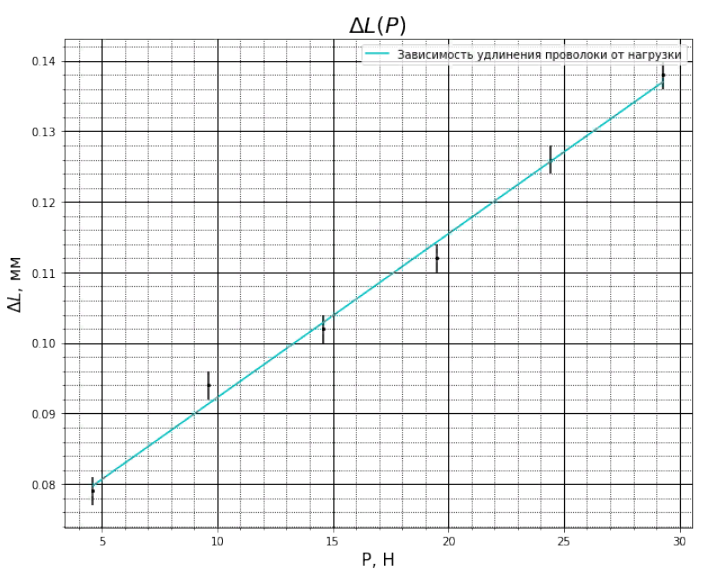
\includegraphics[]{lab131ris4.png}}
\caption{\textit{График зависимости удлинения проволоки от веса нагрузки.}}
\end{figure}

\begin{table}[h!]
\begin{center}
\begin{tabular}{|c|l|c|l|l|}
\hline
\multicolumn{2}{|c|}{Коэффициент   наклона k {[}Н/мм{]}}                                 & \multicolumn{3}{c|}{$430.98$}          \\ \hline
\multicolumn{2}{|c|}{Коэффициент смещения   b {[}мм{]}}                                  & \multicolumn{3}{c|}{$0.069$}           \\ \hline
\multicolumn{2}{|c|}{Погрешность   коэффициента наклона k {[}Н/мм{]}}                    & \multicolumn{3}{c|}{$8.444$}           \\ \hline
\multicolumn{2}{|c|}{Модуль   Юнга {[}Н/м\textasciicircum{}2{]}}                         & \multicolumn{3}{c|}{$1.4\times 10^{11}$} \\ \hline
\multicolumn{2}{|c|}{Погрешность   определения модуля Юнга {[}Н/м\textasciicircum{}2{]}} & \multicolumn{3}{c|}{$3\times 10^{9}$}   \\ \hline
\end{tabular}
\end{center}
\caption{\textit{Итог первого эксперимента.}}
\end{table}

\textbf{ }
\\
\\
\\
\\
\\

\section*{\Large Изгиб балки}



\subsection*{Теоретическая справка}

\begin{figure}[h!]
\center{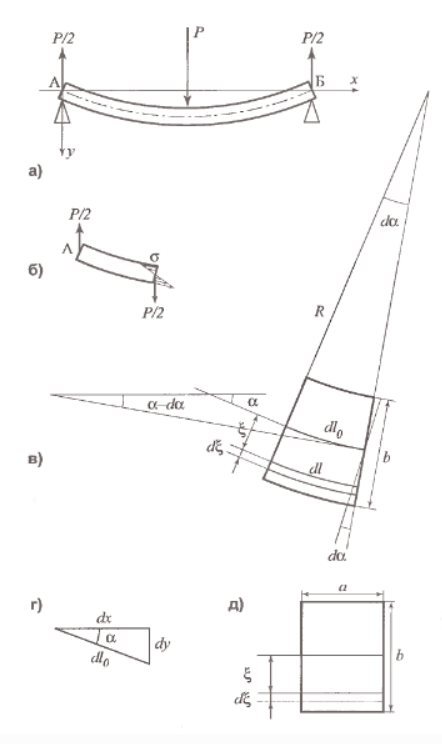
\includegraphics[]{lab131ris3.png}}
\caption{\textit{Изгиб балки.}}
\end{figure}


Рассмотрим деформацию балки. В силу симметричного расположения призм опоры можем считать, что если в центр балки действует сила $P$, то в точках опоры действуют силы $P/2$. Считаем, что напряжения в слоях связаны с их деформацией законом Гука:

\begin{equation}
	\sigma = E \frac{dl-dl_0}{dl_0}.
	\label{form4}
\end{equation}

В выделенном на рисунке элементе балки наклон средней линии на ее длине $dl_0$ меняется от $\alpha$ до $\alpha - d\alpha$. Длину дуги можно выразить через радиус ее кривизны $R$:

\begin{equation}
	dl_0=-Rd\alpha.
	\label{form5}
\end{equation}

Знак минус здесь потому, что $R$ мы считаем положительным, а угол наклона средней линии балки в выбранных на рисунке координатах уменьшается по длине балки. Если $y(x)$ - зависимость, описывающая форму средней линии балки в выбранной системе координат $x,y$, то угол наклона средней линии определяется выражением, соответствующий геометрическому смыслу производной функции:

\begin{equation}
	\frac{dy(x)}{dx}=\tan{\alpha}.
	\label{form6}
\end{equation}

Длину средней линии малого элемента балки можно выразить следующим образом:

\begin{equation}
	dl_0=\sqrt{(dx)^2+(dy)^2}=dx \sqrt{1+(\frac{dy}{dx})^2}.
	\label{form7}
\end{equation}

Из этого же треугольника:

\begin{equation}
	\frac{dx}{dl_0}=\cos{\alpha}.
	\label{form8}
\end{equation}

Дифференцируя $(6)$ по $x$ и пользуясь $(2)$, получаем:

\begin{equation}
	\frac{d^2y}{dx^2}=-(\frac{dl_0}{dx})^3\frac{1}{R}.
	\label{form9}
\end{equation} 

Отсюда и из (7) следует:

\begin{equation}
	\frac{1}{R}=-\frac{y''}{(1+y'^2)^{3/2}}.
	\label{form10}
\end{equation}

Сумма сил упругости, действующих в сечении балки, равна нулю, поэтому их суммарный момент не зависит от положения точки, относительно которой он вычисляется. Выберем эту точку на среденей линии балки, проинтегрируем элементарный момент по $dS$ и получим:

\begin{equation}
	M = \frac{E}{R} I.
	\label{form11}
\end{equation}

$I$ - момент инерции поперечного сечения балки относительно оси, проходящей через среднюю линию балки. Из рисунка видно, что для части былки от $x=0$ до $x$ равновесие обеспечивается равенствомсил, приложенных в точке опоры и в рассматриваемом сечении, а также равенством моментов этих сил и момента, определяемого формулой $(11)$.
Равенство моментов дает:

\begin{equation}
	\frac{EI}{R}=\frac{xP}{2}.
	\label{form12}
\end{equation}

Тогда при малых прогибах $y''\lll 1$ из $(12)$ следует:

\begin{equation}
	y''=-\frac{P}{2EI}x \Rightarrow y'=-\frac{P}{4EI}x^2+C.
	\label{form12}
\end{equation}

$C$ - постоянная, которая определяется из условия симметрии прогиба балки $y'=0$ при $x=l/2$. Тогда:

\begin{equation}
	y'=-\frac{P}{4EI}(x^2-\frac{l^2}{4}) \Rightarrow y=\frac{Px}{48EI}(3l^2-4x^2).
	\label{form13}
\end{equation}

Максимальный прогиб балки, который определяется величиной $y$ при $x=l/2$, равен:

\begin{equation}	
	y_max=\frac{Pl^3}{48EI}.
	\label{form14}
\end{equation}

В случае прямоугольного сечения балки:

\begin{equation}
	I = -\int\limits_{-b/2}^{b/2}{\xi^2 dS}=a\int\limits_{-b/2}^{b/2}{\xi^2 d\xi} = \frac{ab^3}{12}.
	\label{form15}
\end{equation}

Тогда окончательно получаем выражение для модуля Юнга:

\begin{equation}
	E = \frac{Pl^3}{4ab^3y_{max}}.
	\label{form16}
\end{equation}

Здесь $P$ - нагрузка, вызываюшая прогиб стержня, $l$ - расстояние между призмами А и Б, $a$ и $b$ - ширина и высота сечения стержня.



\subsubsection*{Измерения, погрешности и конечный результат}



Измерим указанные геометрические параметры каждой балки и результаты выведем в таблицу 5. В ней же рассчитаем полную погрешность для каждого параметра - она равна корню из суммы квадратов инструментальной и случайной погрешностей:

\begin{table}[h!]
\centering
\scalebox{0.55}{
\begin{tabular}{|c|c|c|c|c|c|c|c|c|}
\hline
\multicolumn{3}{|c|}{\textbf{Деревянная балка 1}}                & \multicolumn{3}{c|}{\textbf{Металлическая балка}}                & \multicolumn{3}{l|}{\textbf{Деревянная балка 2}}                 \\ \hline
\textbf{Длина,   см} & \textbf{Высота, мм} & \textbf{Ширина, мм} & \textbf{Длина,   см} & \textbf{Высота, мм} & \textbf{Ширина, мм} & \textbf{Длина,   см} & \textbf{Высота, мм} & \textbf{Ширина, мм} \\ \hline
50.5                 & 9.17                & 19.1                & 50.5                 & 3.92                & 21.7                & 50.5                 & 10.25               & 19.86               \\ \hline
-                    & 9.12                & 19.3                & -                    & 3.98                & 21.9                & -                    & 10.17               & 20.72               \\ \hline
-                    & 9.13                & 19.1                & -                    & 3.97                & 21.9                & -                    & 10.21               & 20.81               \\ \hline
-                    & 9.03                & 19.3                & -                    & 4.03                & 22.0                & -                    & 10.21               & 20.70               \\ \hline
-                    & 9.05                & 19.5                & -                    & 4.06                & 22.2                & -                    & 9.95                & 20.56               \\ \hline
-                    & 8.97                & 19.6                & -                    & 3.94                & 21.9                & -                    & 9.96                & 20.43               \\ \hline
-                    & 8.9                 & 19.4                & -                    & 3.98                & 21.7                & -                    & 10.04               & 20.40               \\ \hline
-                    & 9.17                & 19.3                & -                    & 3.93                & 21.6                & -                    & 10.15               & 20.45               \\ \hline
-                    & 9.21                & 19.2                & -                    & 3.94                & 21.5                & -                    & 10.19               & 20.51               \\ \hline
-                    & 9.23                & 18.9                & \textbf{-}           & 3.93                & 21.6                & -                    & 10.22               & 20.51               \\ \hline
\multicolumn{3}{|c|}{\textbf{Средние значения}}                  & \multicolumn{3}{c|}{\textbf{Средние значения}}                   & \multicolumn{3}{c|}{\textbf{Средние значения}}                   \\ \hline
50.5                 & 9.10                & 19.27               & 50.5                 & 3.97                & 21.8                & 50.5                 & 10.14               & 20.495              \\ \hline
\multicolumn{3}{|c|}{\textbf{Случайная   погрешность измерения}} & \multicolumn{3}{c|}{\textbf{Случайная   погрешность измерения}}  & \multicolumn{3}{c|}{\textbf{Случайная   погрешность измерения}}  \\ \hline
-                    & 0.108               & 0.206               & -                    & 0.046               & 0.22                & -                    & 0.111               & 0.261               \\ \hline
\multicolumn{3}{|c|}{\textbf{Инструментальная   погрешность}}    & \multicolumn{3}{c|}{\textbf{Инструментальная   погрешность}}     & \multicolumn{3}{c|}{\textbf{Инструментальная   погрешность}}     \\ \hline
0.05                 & 0.005               & 0.005               & 0.05                 & 0.005               & 0.005               & 0.05                 & 0.005               & 0.005               \\ \hline
\multicolumn{3}{|c|}{\textbf{Полная погрешность}}                & \multicolumn{3}{c|}{\textbf{Полная погрешность}}                 & \multicolumn{3}{c|}{\textbf{Полная погрешность}}                 \\ \hline
0.005                & 0.108               & 0.206               & 0.005                & 0.047               & 0.22                & 0.005                & 0.111               & 0.261               \\ \hline
\end{tabular}
}
\caption{\textit{Измерение геометрических параметров балок.}}
\end{table}

\paragraph*{Изучение первой деревянной балки} \textbf{ }
\\

Положим первую деревянную балку на стойку. Снимем зависимость стрелы прогиба $y_{max}$ от величины нагрузки P. Затем сместим точку приложения нагрузки. Перевернем балку и проделаем те же действия. Будем снимать зависимость при возрастании и убывании нагрузки. Результаты выведем в таблице 6.

Построим графики зависимостей величины прогиба от величины нагрузки для каждого из измерений - рисунок 4. На графиках изображены аппроксимирующие прямые, построенные по МНК. Коэффициенты наклона и смещения прямых, их погрешности - отразим в таблице 7.

Получив коэффициент наклона и его погрешность, подставим необходимые данные в формулу (18). Погрешность посчитаем как для степенной зависимости:

	\[\sigma_E=E\times \sqrt{(\frac{\sigma_k}{k})^2+(\frac{\sigma_a}{a})^2+9(\frac{\sigma_b}{b})^2+9(\frac{\sigma_l}{l})^2}. \]

Получим итоговое значение модуля Юнга первой деревянной балки:
	\[E = (669\pm55)\times 10^8  \textbf{Па} \]

\begin{table}[]
\centering
\scalebox{0.65}{
\begin{tabular}{|c|c|c|c|c|}
\hline
\textbf{\begin{tabular}[c]{@{}c@{}}Величина   \\ нагрузки, Н\end{tabular}} & \textbf{\begin{tabular}[c]{@{}c@{}}Прогиб \\ посередине,\\  мм сторона 1\end{tabular}} & \textbf{\begin{tabular}[c]{@{}c@{}}Прогиб\\  со смещением,\\ мм сторона 1\end{tabular}} & \textbf{\begin{tabular}[c]{@{}c@{}}Прогиб\\  посередине балки,\\ мм сторона 2\end{tabular}} & \textbf{\begin{tabular}[c]{@{}c@{}}Прогиб\\ со смещением, мм\\      сторона 2\end{tabular}} \\ \hline
4.5                                                                        & 0.58                                                                                   & 0.56                                                                                    & 0.61                                                                                        & 0.59                                                                                        \\ \hline
9.5                                                                        & 1.25                                                                                   & 1.24                                                                                    & 1.25                                                                                        & 1.23                                                                                        \\ \hline
14.1                                                                       & 1.85                                                                                   & 1.84                                                                                    & 1.86                                                                                        & 1.83                                                                                        \\ \hline
18.7                                                                       & 2.50                                                                                   & 2.43                                                                                    & 2.47                                                                                        & 2.48                                                                                        \\ \hline
14.1                                                                       & 1.88                                                                                   & 1.87                                                                                    & 1.90                                                                                        & 1.89                                                                                        \\ \hline
9.5                                                                        & 1.28                                                                                   & 1.24                                                                                    & 1.28                                                                                        & 1.28                                                                                        \\ \hline
4.5                                                                        & 0.60                                                                                   & 0.55                                                                                    & 0.59                                                                                        & 0.58                                                                                        \\ \hline
\multicolumn{5}{|c|}{\textbf{Усреднение величин}}                                                                                                                                                                                                                                                                                                                                                                                                         \\ \hline
4.5                                                                        & 0.59                                                                                   & 0.56                                                                                    & 0.60                                                                                        & 0.59                                                                                        \\ \hline
9.5                                                                        & 1.27                                                                                   & 1.24                                                                                    & 1.27                                                                                        & 1.26                                                                                        \\ \hline
14.1                                                                       & 1.87                                                                                   & 1.86                                                                                    & 1.88                                                                                        & 1.86                                                                                        \\ \hline
18.7                                                                       & 2.50                                                                                   & 2.43                                                                                    & 2.47                                                                                        & 2.48                                                                                        \\ \hline
\multicolumn{5}{|c|}{\textbf{\begin{tabular}[c]{@{}c@{}}Статистическая погрешность \\ во всех измерениях \\ составляет 0,02 мм\\  - погрешность инструмента.\end{tabular}}}                                                                                                                                                                                                                                                                               \\ \hline
\end{tabular}
}
\caption{\textit{Зависимость величины прогиба от величины нагрузки для первой деревянной балки.}}
\end{table}

\begin{figure}[]
\center{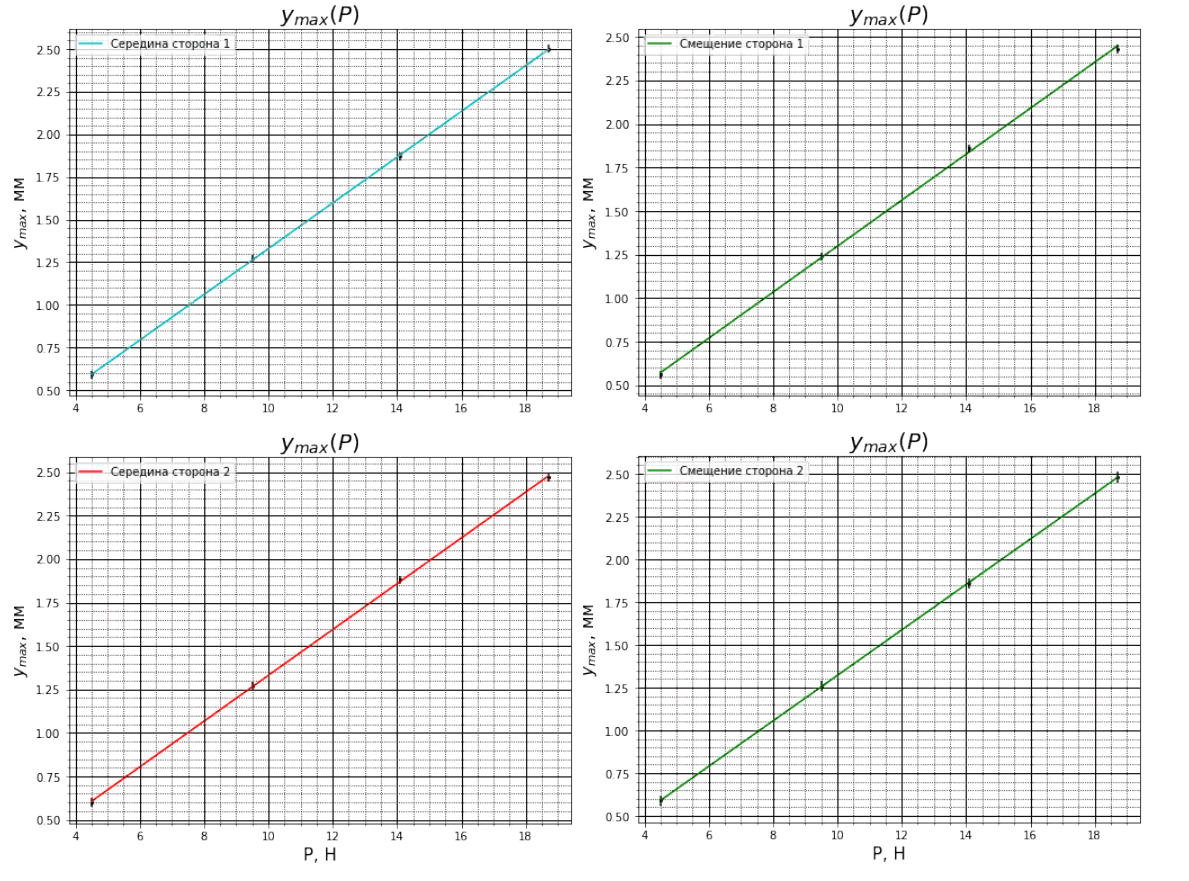
\includegraphics[scale=0.6]{lab131ris5.png}}
\caption{\textit{Графики зависимостей величины прогиба $y_{max}$ от величины нагрузки $P$ для каждого из экспериментов.}}
\end{figure}

\begin{table}[]
\centering
\scalebox{0.8}{
\begin{tabular}{|c|l|l|c|c|}
\hline
\multicolumn{5}{|c|}{\cellcolor[HTML]{FFFFFF}\textbf{МНК   для зависимостей прогиба от нагрузки}}                                  \\ \hline
\multicolumn{3}{|c|}{Коэффициент наклона   для первого эксперимента {[}мм/Н{]}}    & \multicolumn{2}{c|}{0.134}                    \\ \hline
\multicolumn{3}{|c|}{Коэффициент наклона   для второго эксперимента {[}мм/Н{]}}    & \multicolumn{2}{c|}{0.132}                    \\ \hline
\multicolumn{3}{|c|}{Коэффициент наклона   для третьего эксперимента {[}мм/Н{]}}   & \multicolumn{2}{c|}{0.132}                    \\ \hline
\multicolumn{3}{|c|}{Коэффициент наклона   для четвертого эксперимента {[}мм/Н{]}} & \multicolumn{2}{c|}{0.133}                    \\ \hline
\multicolumn{3}{|c|}{Коэффициент смещения   для первого эксперимента {[}мм{]}}     & \multicolumn{2}{c|}{-0.012}                   \\ \hline
\multicolumn{3}{|c|}{Коэффициент смещения   для второго эксперимента {[}мм{]}}     & \multicolumn{2}{c|}{-0.022}                   \\ \hline
\multicolumn{3}{|c|}{Коэффициент смещения   для третьего эксперимента {[}мм{]}}    & \multicolumn{2}{c|}{0.013}                    \\ \hline
\multicolumn{3}{|c|}{Коэффициент смещения   для четвертого эксперимента {[}мм{]}}  & \multicolumn{2}{c|}{-0.007}                   \\ \hline
\multicolumn{5}{|c|}{\cellcolor[HTML]{FFFFFF}\textbf{Погрешность   вычисления коэффициентов МНК}}                                  \\ \hline
\multicolumn{3}{|c|}{Коэффициент наклона   для первого эксперимента {[}мм/Н{]}}    & 0.00889               & 6.63\%                \\ \hline
\multicolumn{3}{|c|}{Коэффициент наклона   для второго эксперимента {[}мм/Н{]}}    & 0.01716               & 13.00\%               \\ \hline
\multicolumn{3}{|c|}{Коэффициент наклона   для третьего эксперимента {[}мм/Н{]}}   & 0.00774               & 5.87\%                \\ \hline
\multicolumn{3}{|c|}{Коэффициент наклона   для четвертого эксперимента {[}мм/Н{]}} & 0.00534               & 4.02\%                \\ \hline
\multicolumn{5}{|c|}{\cellcolor[HTML]{FFFFFF}\textbf{Итоговый   коэффициент наклона {[}мм/Н{]}}}                                   \\ \hline
\multicolumn{3}{|c|}{Усредненный   коэффициент наклона {[}мм/Н{]}}                 & 0.1327                & -                     \\ \hline
\multicolumn{3}{|c|}{Случайная   погрешность вычисления коэффициента наклона}      & 0.0009                & -                     \\ \hline
\multicolumn{3}{|c|}{Статистическая   погрешность вычисления коэффициента наклона} & 0.0098                & -                     \\ \hline
\multicolumn{3}{|c|}{Полная погрешность   вычисления коэффициента наклона}         & 0.0098                & 7.40\%                \\ \hline
\end{tabular}
}
\caption{\textit{Коэффициенты МНК для первой деревянной балки.}}
\end{table}

\paragraph*{Изучение металлической балки} \textbf{ }\\

Положим металлическую балку на стойку. Снимем зависимость стрелы прогиба $y_{max}$ от величины нагрузки P. Затем сместим точку приложения нагрузки. Перевернем балку и проделаем те же действия. Будем снимать зависимость при возрастании и убывании нагрузки. Результаты выведем в таблице 8.

Построим графики зависимостей величины прогиба от величины нагрузки для каждого из измерений - рисунок 5. На графиках изображены аппроксимирующие прямые, построенные по МНК. Коэффициенты наклона и смещения прямых, их погрешности - отразим в таблице 7.

Получив коэффициент наклона и его погрешность, подставим необходимые данные в формулу (18). Погрешность посчитаем как для степенной зависимости:

\[\sigma_E=E\times \sqrt{(\frac{\sigma_k}{k})^2+(\frac{\sigma_a}{a})^2+9(\frac{\sigma_b}{b})^2+9(\frac{\sigma_l}{l})^2}. \]

Получим итоговое значение модуля Юнга первой деревянной балки:
	\[E = (135\pm15)\times 10^8  \textbf{Па}. \]
	
\begin{table}[]
\centering
\scalebox{0.65}{
\begin{tabular}{|c|c|c|c|c|}
\hline
\cellcolor[HTML]{FFFFFF}\textbf{\begin{tabular}[c]{@{}c@{}}Величина \\ нагрузки, Н\end{tabular}} & \textbf{\begin{tabular}[c]{@{}c@{}}Прогиб\\ посередине,\\ мм сторона 1\end{tabular}} & \textbf{\begin{tabular}[c]{@{}c@{}}Прогиб\\ со смещением,\\ мм сторона 1\end{tabular}} & \textbf{\begin{tabular}[c]{@{}c@{}}Прогиб\\ посередине,\\ мм сторона 2\end{tabular}} & \textbf{\begin{tabular}[c]{@{}c@{}}Прогиб \\ со смещением,\\ мм сторона 2\end{tabular}} \\ \hline
4.5                                                                                              & 1.01                                                                                 & 0.99                                                                                   & 1.03                                                                                 & 0.96                                                                                    \\ \hline
9.5                                                                                              & 2.19                                                                                 & 2.10                                                                                   & 2.30                                                                                 & 2.15                                                                                    \\ \hline
14.1                                                                                             & 3.19                                                                                 & 3.25                                                                                   & 3.35                                                                                 & 3.23                                                                                    \\ \hline
18.7                                                                                             & 4.28                                                                                 & 4.31                                                                                   & 4.54                                                                                 & 4.29                                                                                    \\ \hline
14.1                                                                                             & 3.25                                                                                 & 3.26                                                                                   & 3.49                                                                                 & 3.35                                                                                    \\ \hline
9.5                                                                                              & 2.17                                                                                 & 2.25                                                                                   & 2.45                                                                                 & 2.35                                                                                    \\ \hline
4.5                                                                                              & 1.01                                                                                 & 1.16                                                                                   & 1.22                                                                                 & 1.10                                                                                    \\ \hline
\multicolumn{5}{|c|}{\textbf{Усреднение величин}}                                                                                                                                                                                                                                                                                                                                                                                                                 \\ \hline
4.5                                                                                              & 1.01                                                                                 & 1.08                                                                                   & 1.13                                                                                 & 1.03                                                                                    \\ \hline
9.5                                                                                              & 2.18                                                                                 & 2.18                                                                                   & 2.38                                                                                 & 2.25                                                                                    \\ \hline
14.1                                                                                             & 3.22                                                                                 & 3.26                                                                                   & 3.42                                                                                 & 3.29                                                                                    \\ \hline
18.7                                                                                             & 4.28                                                                                 & 4.31                                                                                   & 4.54                                                                                 & 4.29                                                                                    \\ \hline
\multicolumn{5}{|c|}{\textbf{\begin{tabular}[c]{@{}c@{}}Статистическая погрешность\\ во всех измерениях \\ составляет 0,02 мм\\ - погрешность инструмента.\end{tabular}}}                                                                                                                                                                                                                                                                                         \\ \hline
\end{tabular}
}
\caption{\textit{Зависимость величины прогиба от величины нагрузки для первой деревянной балки.}}
\end{table}

\begin{figure}[]
\center{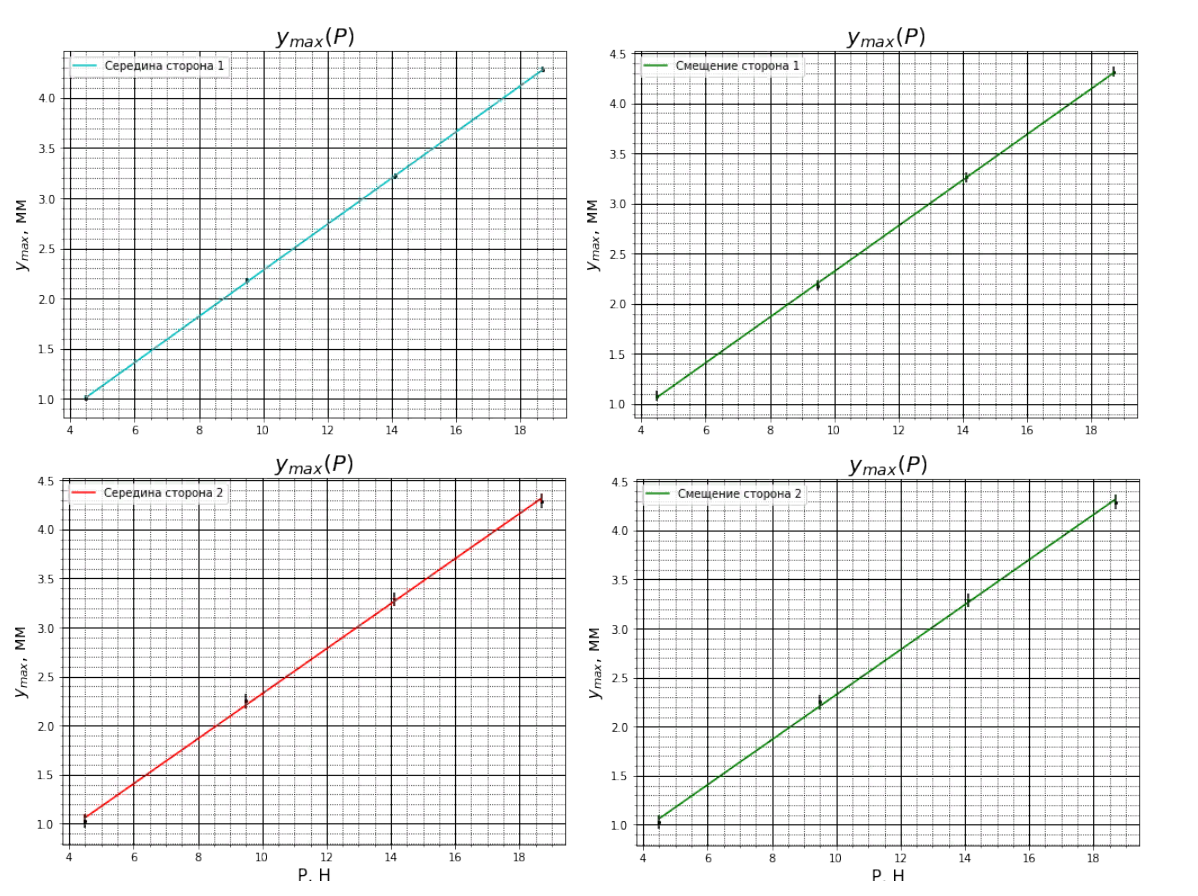
\includegraphics[scale=0.6]{lab131ris6.png}}
\caption{\textit{Графики зависимостей величины прогиба $y_{max}$ от величины нагрузки $P$ для каждого из экспериментов.}}
\end{figure}

\begin{table}[h!]
\centering
\scalebox{0.7}{
\begin{tabular}{
>{\columncolor[HTML]{FFFFFF}}c |
>{\columncolor[HTML]{FFFFFF}}l |
>{\columncolor[HTML]{FFFFFF}}l |
>{\columncolor[HTML]{FFFFFF}}c |
>{\columncolor[HTML]{FFFFFF}}c |}
\hline
\multicolumn{5}{|c|}{\cellcolor[HTML]{FFFFFF}\textbf{МНК   для зависимостей прогиба от нагрузки}}                                                                      \\ \hline
\multicolumn{3}{|c|}{\cellcolor[HTML]{FFFFFF}Коэффициент наклона   для первого эксперимента {[}мм/Н{]}}    & \multicolumn{2}{c|}{\cellcolor[HTML]{FFFFFF}0.229899497}  \\ \hline
\multicolumn{3}{|c|}{\cellcolor[HTML]{FFFFFF}Коэффициент наклона   для второго эксперимента {[}мм/Н{]}}    & \multicolumn{2}{c|}{\cellcolor[HTML]{FFFFFF}0.228122757}  \\ \hline
\multicolumn{3}{|c|}{\cellcolor[HTML]{FFFFFF}Коэффициент наклона   для третьего эксперимента {[}мм/Н{]}}   & \multicolumn{2}{c|}{\cellcolor[HTML]{FFFFFF}0.238837042}  \\ \hline
\multicolumn{3}{|c|}{\cellcolor[HTML]{FFFFFF}Коэффициент наклона   для четвертого эксперимента {[}мм/Н{]}} & \multicolumn{2}{c|}{\cellcolor[HTML]{FFFFFF}0.229361091}  \\ \hline
\multicolumn{3}{|c|}{\cellcolor[HTML]{FFFFFF}Коэффициент смещения   для первого эксперимента {[}мм{]}}     & \multicolumn{2}{c|}{\cellcolor[HTML]{FFFFFF}-0.017324121} \\ \hline
\multicolumn{3}{|c|}{\cellcolor[HTML]{FFFFFF}Коэффициент смещения   для второго эксперимента {[}мм{]}}     & \multicolumn{2}{c|}{\cellcolor[HTML]{FFFFFF}0.038463747}  \\ \hline
\multicolumn{3}{|c|}{\cellcolor[HTML]{FFFFFF}Коэффициент смещения   для третьего эксперимента {[}мм{]}}    & \multicolumn{2}{c|}{\cellcolor[HTML]{FFFFFF}0.073106604}  \\ \hline
\multicolumn{3}{|c|}{\cellcolor[HTML]{FFFFFF}Коэффициент смещения   для четвертого эксперимента {[}мм{]}}  & \multicolumn{2}{c|}{\cellcolor[HTML]{FFFFFF}0.031475233}  \\ \hline
\multicolumn{5}{|c|}{\cellcolor[HTML]{FFFFFF}\textbf{Погрешность   вычисления коэффициентов МНК}}                                                                      \\ \hline
\multicolumn{3}{|c|}{\cellcolor[HTML]{FFFFFF}Коэффициент наклона   для первого эксперимента {[}мм/Н{]}}    & 0.00928                      & 4.04\%                     \\ \hline
\multicolumn{3}{|c|}{\cellcolor[HTML]{FFFFFF}Коэффициент наклона   для второго эксперимента {[}мм/Н{]}}    & 0.01951                      & 8.55\%                     \\ \hline
\multicolumn{3}{|c|}{\cellcolor[HTML]{FFFFFF}Коэффициент наклона   для третьего эксперимента {[}мм/Н{]}}   & 0.02721                      & 11.39\%                    \\ \hline
\multicolumn{3}{|c|}{\cellcolor[HTML]{FFFFFF}Коэффициент наклона   для четвертого эксперимента {[}мм/Н{]}} & 0.03880                      & 16.91\%                    \\ \hline
\multicolumn{5}{|c|}{\cellcolor[HTML]{FFFFFF}\textbf{Итоговый   коэффициент наклона {[}мм/Н{]}}}                                                                       \\ \hline
\multicolumn{3}{|c|}{\cellcolor[HTML]{FFFFFF}Усредненный   коэффициент наклона {[}мм/Н{]}}                 & 0.2316                       & -                          \\ \hline
\multicolumn{3}{|c|}{\cellcolor[HTML]{FFFFFF}Случайная   погрешность вычисления коэффициента наклона}      & 0.0043                       & -                          \\ \hline
\multicolumn{3}{|c|}{\cellcolor[HTML]{FFFFFF}Статистическая   погрешность вычисления коэффициента наклона} & 0.0237                       & -                          \\ \hline
\multicolumn{3}{|c|}{\cellcolor[HTML]{FFFFFF}Полная погрешность   вычисления коэффициента наклона}         & 0.0241                       & 10.40\%                    \\ \hline
\end{tabular}
}
\caption{\textit{Коэффициенты МНК для металлической балки.}}
\end{table}


\paragraph*{Изучение второй деревянной
 балки} \textbf{ }\\

Положим металлическую балку на стойку. Снимем зависимость стрелы прогиба $y_{max}$ от величины нагрузки P. Затем сместим точку приложения нагрузки. Перевернем балку и проделаем те же действия. Будем снимать зависимость при возрастании и убывании нагрузки. Результаты выведем в таблице 10.

Построим графики зависимостей величины прогиба от величины нагрузки для каждого из измерений - рисунок 6. На графиках изображены аппроксимирующие прямые, построенные по МНК. Коэффициенты наклона и смещения прямых, их погрешности - отразим в таблице 7.

Получив коэффициент наклона и его погрешность, подставим необходимые данные в формулу (18). Погрешность посчитаем как для степенной зависимости:

\[\sigma_E=E\times \sqrt{(\frac{\sigma_k}{k})^2+(\frac{\sigma_a}{a})^2+9(\frac{\sigma_b}{b})^2+9(\frac{\sigma_l}{l})^2}. \]

Получим итоговое значение модуля Юнга первой деревянной балки:
	\[E = (447\pm38)\times 10^8  \textbf{Па}. \]
	
\section*{\center\text{Вывод}}

Изучена зависимость между напряжением и деформацией (закон Гука) для двух простейших напряженных состояний упругих тел: одноосного растяжения и чистого изгиба; по результатам измерений были вычислены модули Юнга для каждого из материалов.  
	
\begin{table}[h!]
\centering
\scalebox{0.65}{
\begin{tabular}{|c|c|c|c|c|}
\hline
\cellcolor[HTML]{FFFFFF}\textbf{\begin{tabular}[c]{@{}c@{}}Величина\\ нагрузки, Н\end{tabular}} & \textbf{\begin{tabular}[c]{@{}c@{}}Прогиб \\ посередине,\\ мм сторона 1\end{tabular}} & \textbf{\begin{tabular}[c]{@{}c@{}}Прогиб\\  со смещением, \\ мм сторона 1\end{tabular}} & \textbf{\begin{tabular}[c]{@{}c@{}}Прогиб \\ посередине,\\ мм сторона 2\end{tabular}} & \textbf{\begin{tabular}[c]{@{}c@{}}Прогиб \\ со смещением, \\ мм сторона 2\end{tabular}} \\ \hline
4.5                                                                                             & 0.58                                                                                  & 0.56                                                                                     & 0.52                                                                                  & 0.54                                                                                     \\ \hline
9.5                                                                                             & 1.36                                                                                  & 1.27                                                                                     & 1.22                                                                                  & 1.24                                                                                     \\ \hline
14.1                                                                                            & 1.95                                                                                  & 1.89                                                                                     & 1.85                                                                                  & 1.83                                                                                     \\ \hline
18.7                                                                                            & 2.63                                                                                  & 2.53                                                                                     & 2.49                                                                                  & 2.50                                                                                     \\ \hline
14.1                                                                                            & 2.01                                                                                  & 1.93                                                                                     & 1.89                                                                                  & 1.91                                                                                     \\ \hline
9.5                                                                                             & 1.38                                                                                  & 1.32                                                                                     & 1.31                                                                                  & 1.32                                                                                     \\ \hline
4.5                                                                                             & 0.69                                                                                  & 0.65                                                                                     & 0.65                                                                                  & 0.68                                                                                     \\ \hline
\multicolumn{5}{|c|}{\textbf{Усреднение величин}}                                                                                                                                                                                                                                                                                                                                                                                                                     \\ \hline
4.5                                                                                             & 0.64                                                                                  & 0.61                                                                                     & 0.59                                                                                  & 0.61                                                                                     \\ \hline
9.5                                                                                             & 1.37                                                                                  & 1.30                                                                                     & 1.27                                                                                  & 1.28                                                                                     \\ \hline
14.1                                                                                            & 1.98                                                                                  & 1.91                                                                                     & 1.87                                                                                  & 1.87                                                                                     \\ \hline
18.7                                                                                            & 2.63                                                                                  & 2.53                                                                                     & 2.49                                                                                  & 2.50                                                                                     \\ \hline
\multicolumn{5}{|c|}{\textbf{\begin{tabular}[c]{@{}c@{}}Статистическая погрешность \\ во всех измерениях\\  составляет 0,02 мм\\  - погрешность инструмента.\end{tabular}}}                                                                                                                                                                                                                                                                                           \\ \hline
\end{tabular}
}
\caption{\textit{Зависимость величины прогиба от величины нагрузки для второй деревянной балки.}}
\end{table}

\begin{figure}[]
\center{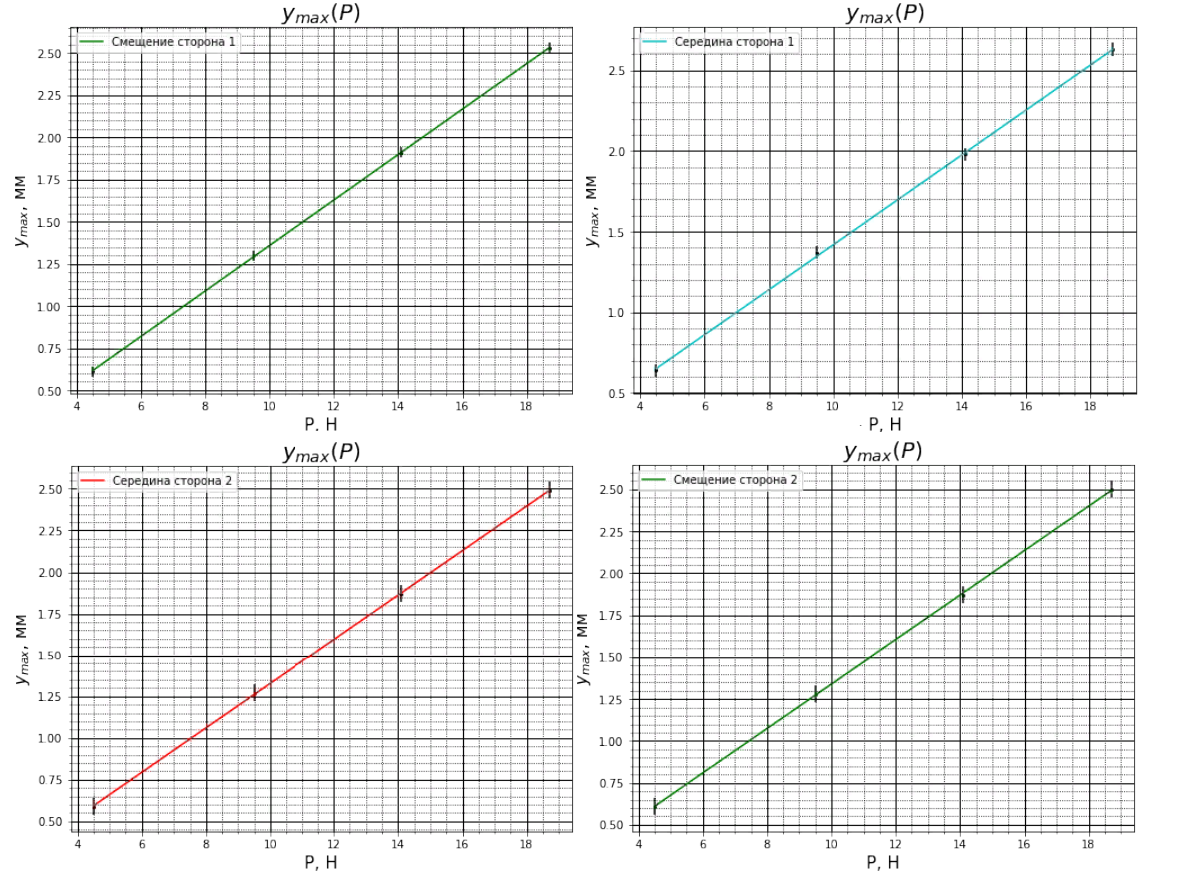
\includegraphics[scale=0.6]{lab131ris7.png}}
\caption{\textit{Графики зависимостей величины прогиба $y_{max}$ от величины нагрузки $P$ для каждого из экспериментов.}}
\end{figure}

\begin{table}[h!]
\centering
\scalebox{0.7}{
\begin{tabular}{|
>{\columncolor[HTML]{FFFFFF}}c |
>{\columncolor[HTML]{FFFFFF}}l |
>{\columncolor[HTML]{FFFFFF}}l |
>{\columncolor[HTML]{FFFFFF}}c |
>{\columncolor[HTML]{FFFFFF}}c |}
\hline
\multicolumn{5}{|c|}{\cellcolor[HTML]{FFFFFF}\textbf{МНК   для зависимостей прогиба от нагрузки}}                                                                      \\ \hline
\multicolumn{3}{|c|}{\cellcolor[HTML]{FFFFFF}Коэффициент наклона   для первого эксперимента {[}мм/Н{]}}    & \multicolumn{2}{c|}{\cellcolor[HTML]{FFFFFF}0.139447236}  \\ \hline
\multicolumn{3}{|c|}{\cellcolor[HTML]{FFFFFF}Коэффициент наклона   для второго эксперимента {[}мм/Н{]}}    & \multicolumn{2}{c|}{\cellcolor[HTML]{FFFFFF}0.134978464}  \\ \hline
\multicolumn{3}{|c|}{\cellcolor[HTML]{FFFFFF}Коэффициент наклона   для третьего эксперимента {[}мм/Н{]}}   & \multicolumn{2}{c|}{\cellcolor[HTML]{FFFFFF}0.133488873}  \\ \hline
\multicolumn{3}{|c|}{\cellcolor[HTML]{FFFFFF}Коэффициент наклона   для четвертого эксперимента {[}мм/Н{]}} & \multicolumn{2}{c|}{\cellcolor[HTML]{FFFFFF}0.132627423}  \\ \hline
\multicolumn{3}{|c|}{\cellcolor[HTML]{FFFFFF}Коэффициент смещения   для первого эксперимента {[}мм{]}}     & \multicolumn{2}{c|}{\cellcolor[HTML]{FFFFFF}0.023467337}  \\ \hline
\multicolumn{3}{|c|}{\cellcolor[HTML]{FFFFFF}Коэффициент смещения   для второго эксперимента {[}мм{]}}     & \multicolumn{2}{c|}{\cellcolor[HTML]{FFFFFF}0.008251974}  \\ \hline
\multicolumn{3}{|c|}{\cellcolor[HTML]{FFFFFF}Коэффициент смещения   для третьего эксперимента {[}мм{]}}    & \multicolumn{2}{c|}{\cellcolor[HTML]{FFFFFF}-0.006819813} \\ \hline
\multicolumn{3}{|c|}{\cellcolor[HTML]{FFFFFF}Коэффициент смещения   для четвертого эксперимента {[}мм{]}}  & \multicolumn{2}{c|}{\cellcolor[HTML]{FFFFFF}0.013259153}  \\ \hline
\multicolumn{5}{|c|}{\cellcolor[HTML]{FFFFFF}\textbf{Погрешность   вычисления коэффициентов МНК}}                                                                      \\ \hline
\multicolumn{3}{|c|}{\cellcolor[HTML]{FFFFFF}Коэффициент наклона   для первого эксперимента {[}мм/Н{]}}    & 0.01713                      & 12.28\%                    \\ \hline
\multicolumn{3}{|c|}{\cellcolor[HTML]{FFFFFF}Коэффициент наклона   для второго эксперимента {[}мм/Н{]}}    & 0.00701                      & 5.20\%                     \\ \hline
\multicolumn{3}{|c|}{\cellcolor[HTML]{FFFFFF}Коэффициент наклона   для третьего эксперимента {[}мм/Н{]}}   & 0.00646                      & 4.84\%                     \\ \hline
\multicolumn{3}{|c|}{\cellcolor[HTML]{FFFFFF}Коэффициент наклона   для четвертого эксперимента {[}мм/Н{]}} & 0.00972                      & 7.33\%                     \\ \hline
\multicolumn{5}{|c|}{\cellcolor[HTML]{FFFFFF}\textbf{Итоговый коэффициент   наклона {[}мм/Н{]}}}                                                                       \\ \hline
\multicolumn{3}{|c|}{\cellcolor[HTML]{FFFFFF}Усредненный   коэффициент наклона {[}мм/Н{]}}                 & 0.1351                       & -                          \\ \hline
\multicolumn{3}{|c|}{\cellcolor[HTML]{FFFFFF}Случайная   погрешность вычисления коэффициента наклона}      & 0.0026                       & -                          \\ \hline
\multicolumn{3}{|c|}{\cellcolor[HTML]{FFFFFF}Статистическая   погрешность вычисления коэффициента наклона} & 0.0101                       & -                          \\ \hline
\multicolumn{3}{|c|}{\cellcolor[HTML]{FFFFFF}Полная погрешность   вычисления коэффициента наклона}         & 0.0104                       & 7.71\%                     \\ \hline
\end{tabular}
}
\caption{\textit{Коэффициенты МНК для металлической балки.}}
\end{table}



\end{document}